\chapter{Dictionaries}
%\thispagestyle{empty}
In section \ref{sec:dicts} we give a general definition of dictionaries 
as indexed sets of signal atoms with unknown structure of the atoms.
Dictionaries for sparse coding of images are indexed collection of vectors with
discrete pixel data. A linear combination of a sparse selection of those
discrete pixel atoms are used to reconstruct signals. 

\section{Structure}
But atoms are not just made up of random pixel data. Dictionary atoms should
capture structures that are useful for sparse coding. Just picking a few of
them should lead to a good reconstruction. 

Finding the right structures for a specific signal is a complex task.
The two main strategies for the generation of the dictionaries are design and
learning.

\subsection{Designed atoms}
The basis transformations first presented in\ref{sec:history} can also
be interpreted as atoms of discrete pixel data. This can be atoms with only
locality in frequency like cosine from DCT or atoms with both locality in time
and frequency like wavelts. Figure \ref{fig:generated_atoms}
shows some examples for such dictionaries. 

%\paragraph{cosine}
%\paragraph{wavelets}
%\paragraph{curvelets/contourlets/bandelets}
%\Todo{}

\begin{figure}
\centering
\subfloat[cosine]{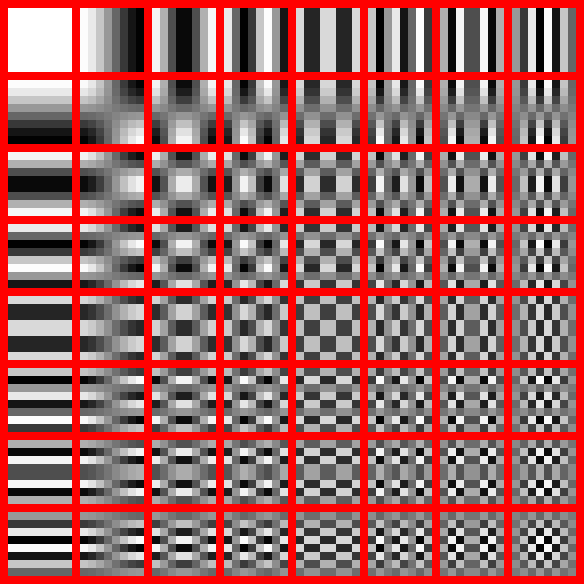
\includegraphics[width =
0.3\textwidth]{images/dct.png}}
\hspace{5mm}
\subfloat[haar wavelets]{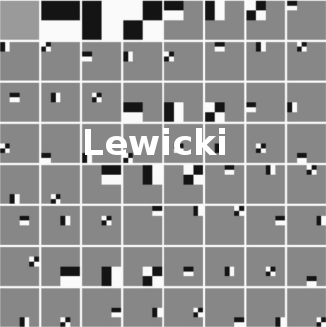
\includegraphics[width =
0.3\textwidth]{images/haar.png}}
\hspace{5mm}
\subfloat[gabor wavelts]{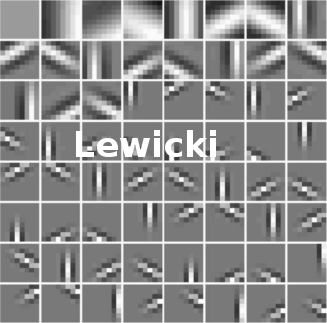
\includegraphics[width =
0.3\textwidth]{images/gabor.png}}
\caption{generated bases}

\label{fig:generated_atoms}
\end{figure}

\subsection{Learned atoms}
%\begin{quotation}
%A computer program is said to learn from experience E with respect to
%some class of tasks T and performance measure P, if its performance at tasks in
%T, as measured by P, improves with experience E.\footnote{Tom M. Mitchell}
%\end{quotation}
Recent research\cite{Chen1998,Aharon2006,Mairal2010} has shown that learned
dictionaries show better compression quality than small analytic
dictionaries. Rather than selecting an appropriate mathematical construct that
can reconstruct a certain group of signals close enough the data, a subset of
the data or similar data is used as a training set to learn the dictionary
itself.
%Besides the construction of dictionaries from mathematical functions, machine
%learning can also be used to to generate dictionaries. 
Machine learning is such a process that is used to learn essential structures
from empirical data. In the case of dictionaries for sparse coding these
empirical data are sets of signals which are feed as training data into machine
learning algorithms.

Principal component analysis (PCA) can be used as an approach to find such
dictionary atoms. As the principal components are orthogonal to each other PCA
can only find a number atoms of atoms that is lower or equal to the dimension of
the signal. When we want to use these atoms for sparse coding we are limited to
a small range of possible atoms.

\paragraph{Redundancy} Unlike the PCA approach,
dictionary atoms learned with machine learning methods are not necessarily
orthogonal. In fact one benefit of the machine learning approach is to be able
to learn over-complete dictionaries with non-orthogonal basis atoms. This is
where redundancy enters the game of constructing dictionaries. Not in a way
where multiple instance of the same element are part of the dictionary but in
form of additional elements that resemble a composition of other elements from
the dictionary. This can lead to less required atoms and more sparseness of the
coefficient vector $\alpha$ when sparse coding signals. Now a single atom can
achieve the same reconstruction as a former combination of several orthogonal
basis elements. 
Nevertheless redundancy can also be applied to the designed
dictionaries. For example by adding rotated cosine elements to a dictionary with
a default configuration of DCT basis elements.


\section{Learning}
%\cite{Olshausen1997,Lewicki2000,Aharon2006}
In the last decade several learning algorithms for over-complete dictionaries
have been proposed. The basic concept of following algorithms for learning
redundant dictionaries is to alter a initial start dictionary in a way that it
can sparsely reconstruct a set of training data with minimal error. 

\begin{align} 
D = \argmax_{D} \sum_{i=0}^n \max_{x_i} P(x,D)
\end{align}
L loss function, E error function
\begin{align} 
D = \argmin_{D} \sum_{i=0}^n L(x_i,D)
\end{align}

\begin{align} 
\argmin_{D,\alpha} \sum_{i}
\lVert x_i - D\alpha_i \rVert^{2}_{2}  +  \lambda \lVert \alpha_i
\rVert_{0,1,2}
\end{align}
There are two major groups of algorithms for learning redundant dictionaries for
sparse coding. Learning dictionary elements from a fixed batch of training
signals and learning dictionary elements from a constant flow of data. The later
enables to start the learning process before the actual training data is known.
An advantage that is used to learn from live data, for example video and audio,
or big data sets that would challenge the limits of a batch bases algorithm. We
now introduce some of the most popular algorithms for both ways of learning.

\subsection{Batch algorithms}
Batch algorithms learn over-complete dictionaries from fixed batches of
training data. We present some of the most popular of these algorithms.

\paragraph{Method of optimal directions (MOD)}
Presented by Engan et al. in 1999\cite{Engan1999a} 

\paragraph{ILS-DLA}
In 2007 Engan et al.\cite{Engan2007} presented another algorithm by   


\subsubsection{K-SVD}
\label{sec:k-svd}
One of the most popular batch algorithms is the K-SVD presented by
Aharon et al. in 2006\cite{Aharon2006}. The algorithm learns a dictionary $D$
from a set of training samples $X$ by solving:
\begin{equation*}
\min_{D,A} \lVert X - DA \rVert^{2}_{F} \textrm{ s.t. }
\forall i : \lVert \alpha_i \rVert_{0} \leq L
\end{equation*}
At the beginning the dictionary $D$ gets initialized with either random data or
a random selection of elements from the training set. The main part of the
algorithm consists of two step which are repeated for a fixed number of $T$
iterations or until convergence of $D$. In the first step all samples of
training $X$ are sparse coded with the current dictionary $D$. In the second
step every dictionary atom $d_j$ of $D$ is altered in a way that the
reconstruction error of $X$ is minimized. 
\begin{equation*}
\min_{d_j,a_j} \lVert d_ja_j - E_j \rVert^{2}_{F} \textrm{ with }
E_j = \sum_{l\neq j} d_la_l^T - X
\end{equation*} 
The trick of update step is to consider only the signal in $X$ which use the
atom $d_j$. The problem gets then solved with a \emph{Singular Value
Decomposition (SVD)}. 
%The name K-SVD comes from $k$ times application of SVD in the update process
%(line \label{alg:k-svd_start} till line \ref{alg:k-svd_end} in algorithm
%\ref{alg:k-svd}).
The \prettyref{alg:k-svd} illustrates this procedure. 

\begin{algorithm}[H]
\caption{K-SVD}
\label{alg:k-svd}
\begin{algorithmic}[1]
\REQUIRE $X \in \mathbb{R}^{m \times k}, \lambda \in
\mathbb{R}, D_0 \in \mathbb{R}^{m \times p}, T \in \mathbb{N}$
\STATE $A \gets D_0$
\FOR {$t = 1$ to $T$}
\STATE sparse code every $x_i$ in $X$ with $D$:
\begin{equation}
\alpha = \argmin_{\alpha}\lVert
x_t - D\alpha\rVert_2^2 \text{ s.t.} \lVert\alpha\rVert_0 \leq L
\end{equation}
\FOR {$j = 1$ to $p$}\label{alg:k-svd_start}
\STATE $D_j \gets 0$
\STATE $I \gets \{ i : \forall i : A_{j,i} \neq 0 \}$
\STATE $E \gets X_I - DA_I$
\STATE $\{ d,g\} \gets \argmin_{d,g} \lVert E- dg^T \rVert_F^{2}$ s. t. $\lVert
d
\rVert_{2} = 1$
\STATE $D_j \gets d$
\STATE $A_{j,I} \gets g^T$
\ENDFOR\label{alg:k-svd_end}
\ENDFOR
\RETURN $D$
\end{algorithmic}
\end{algorithm}
\Todo{optional: k-svd modifications}

\subsection{On-line algorithms}
In 2009 new training algorithms were presented that enabled on-line learning of
dictionaries. In contrast to batch learning algorithms with a fixed training set
the new approaches enable learning with a constant flow of training data. This
is good for very large training sets or training data that is unknown at the
start of the training process.

\paragraph{Recursive least-square dictionary learning algorithm (ILS-DLA)}
The algorithm was presented by Engan et al. in 2010\cite{Engan2010} and is a
recursive the a modified version of the ILS-DLA algorithm.


\subsubsection{Online dictionary learning}
\label{sec:mairal}
In 2010 Mairal et. al.\cite{Mairal2010} proposed an on-line approach which from
now on we will call \trainDL. The algorithm presented by Mairal et
al.\cite{Mairal2010} is ... 
stochastic approximations 
It is a minimization that uses block-coordinate descent with warm restart for
the dictionary update step.
Like the K-SVD the algorithm learns a dictionary $D$ from a set of training
samples $X$ and starts with a dictionary $D$ with random data or a random
selection of elements from the training set. 
First sparse code a signal  1

Solving $ $ 
only store $A$ and $B$ 
As it pretends to scale up to large datasets of millions of training samples
and being suitable for a large range of learning problems.
Does it scale up to big dictionaries?
samples\cite{Mairal2010}
\begin{algorithm}[H]
\caption[\trainDL]{Online dictionary learning\cite{Mairal2010}}
\label{alg:trainDL}
\begin{algorithmic}[1]
\REQUIRE $x \in \mathbb{R}^{m \times k},  p \left( x \right), \lambda \in \mathbb{R}, D_0 \in \mathbb{R}^{m \times p}, T \in \mathbb{N}$
\STATE $A_0 \in \mathbb{R}^{p \times p} \gets  0, B_0 \in \mathbb{R}^{m \times p}\gets 0$
\FOR {$t = 1$ to $T$}
\STATE Draw $x$ from p(x).
\STATE Sparse code:
\begin{align*} 
\alpha_t \equiv \argmin_{\alpha\in\mathbb{R}^{p}}  \lVert x_t - D_t\alpha \rVert^{2}_{2}  +  \lambda \lVert \alpha \rVert_{1}
\end{align*}

\STATE $A_t \gets A_{t-1} + \alpha_t\alpha_t^T$\label{alg:Aupdate}
\STATE $B_t \gets B_{t-1} + x_t\alpha_t^T$\label{alg:Bupdate}
\STATE Compute $D_t$ using \prettyref{alg:update}, with $D_{t-1}$ as warm restart 
\begin{equation}
\begin{split}
D_t  & \equiv \argmin_{D \in \mathbb{R}^{m x k}}  \frac{1}{t} \sum_{i=1}^t
\left( \frac{1}{2} \lVert x_i - D\alpha_i \rVert^{2}_{2}  +  \lambda \lVert
\alpha_i \rVert_{1} \right) \\
& = \argmin_{D \in \mathbb{R}^{m x k}}  \frac{1}{t} \sum_{i=1}^t
\left( \frac{1}{2} Tr(D^TDA_t) - Tr(D^TB_t)\right) \label{eq:update}
\end{split}
\end{equation}
 
\ENDFOR
\RETURN $D_T$
\end{algorithmic}
\end{algorithm}


\begin{algorithm}[H]
\caption{Dictionary Update}
\label{alg:update}
\begin{algorithmic}[1]
\REQUIRE $D=[d_1,...,d_p] \in \mathbb{R}^{m \times p}, A=[a_1,...,a_p] \in \mathbb{R}^{p \times p}, B=[b_1,...,b_p] \in \mathbb{R}^{m \times p}$
\REPEAT
\FOR {$j = 1$ to $p$}
\STATE update j-th column to optimize for \prettyref{eq:update}:
\begin{align*}
u_j \gets \frac{1}{A[j,j]}\left(b_j-Da_j\right)+d_j \\
d_j \gets \frac{1}{\max\left(\lVert u_j \rVert_2,1\right)} u_j
\end{align*}

\ENDFOR
\UNTIL convergence 
\RETURN $D$
\end{algorithmic}
\end{algorithm}
Mairal et al. describe several modification to their algorithm to improve speed
and convergence. One speed optimization is to sparse code mini-batches of $n$
signal samples instead of a single signal sample in each iteration. This
modification leads to line \ref{alg:Aupdate} and line \ref{alg:Bupdate}
becoming:
\begin{align}
A_t \gets A_{t-1} + \frac{1}{n}\sum_{i=1}^{n}\alpha_{t,i}\alpha_{t,i}^T\\
B_t \gets B_{t-1} + \frac{1}{n}\sum_{i=1}^{n}x_{t,i}\alpha_{t,i}^T
\end{align}

%$A_0  \gets tI$ and $B_0 \gets tD$




\subsection{Learning for the Task}
\label{sec:learnForTheTask}
``Please do not use the wrong dictionaries...''\footnote
mentions Guillermo Sapiro in his talk at the \emph{MIT CSAIL}
It has been shown that learning specific for certain tasks can lead to the
best results. Based on this finding we will concentrate on a
specific class. We will focus on natural images from large image databases.
This means typicaly 1+ mega-pixel images with 3-channel RGB data found on image
hosting services such as flickr.com, twitpic.com, picasa.com among others.


\section{Related work}
\label{sec:related_dictionarie}
%Current research is primary concentrating on other tasks. 
%Like ... related work :)
%\begin{description}

\paragraph{Texture synthesis}\cite{Peyre2008}

\paragraph{Vector quantization}

\paragraph{Epitomes} In 2008 Wang et al.\cite{Wang2008a} presented
an approach that factors repeated content in images. The algorithm generates 
a map of affine transformations and an epitome atlas map with ... . The
epitomes are also a sort of dictionary and the affine transformation matrices
the corresponding .. The technique is used for real-time synthesis of textures
with low memory consumption and  fast reconstruction in hardware via pixel
shaders. They also presented some experiments for unified epitomes for
collection of images and possible application for larger sets of images. 
%The algorithm so caled eptimes
%Factoring repeated content\cite{factor_image}

\paragraph{Training with a neural network} In his masters thesis 
\cite{Krizhevsky2009}
%Learning Multiple Layers of Features from Tiny Images
Using an neural network to learn image basis from a large set of tiny images.
The resulting basis elements look like ...

\paragraph{Compression of facial images}
In 2008 Bryt and Elad \cite{Bryt2008} 
\paragraph{Compression} \cite{Lewicki1999,Murray2006}  
Another example of a more specific compression task is the
work on facial image compression by Bryt and Elad \cite{Bryt2008}. 
They took a collection of black and white facial images. Aligned them and
learned  

\paragraph{Multi-scale dictionaries}
Rather than encoding uniform segments of a bigger signal this technique
encodes different sized blocks (multiple times of the default block size). The
idea is that aligned smooth regions with low variance can be can be combined
encoded as one signal rather than for example four.\cite{Mairal2007}

\Todo{picture with different scales}

\paragraph{Classification} \cite{?} validation of fake paintings. 
\cite{?} classification of object by learning individual dictionaries for each
object group. Additional examples for sparse coding  being used for
classification tasks can be found in
\cite{Raina2007,BradleyBagnel2009,Mairal2008,Mairal2008b,Bar2009,Yang2009}.


%\paragraph{Multi-channel}
%When dealing with multi-channel data (e.g. RGB images) each channel can be
%coded separate or as a concatenation of each signal into a single one. These
%approaches can lead to color bleeding \cite{mairal08sparse} \Todo{add picture}
%Fortunately this problem vanishes with big dictionaries and large training
%sets. \cite{mairal08sparse} Nevertheless a solution would be to add a
%constraint to the sparse coding that pays attention the correlation of the
%channels. \Todo{add formula from paper}

\paragraph{Double sparsity}
Instead of directly using a collection of trained atoms as dictionary
elements. This approach uses sparse coding to encode the signals of a bigger
dictionary with the help of a smaller on.\cite{Rubinstein2009} 
\Todo{formula $B$ .. basis, $A$ sparse matrix, $D=BA$ ...}


\paragraph{Hierarchy}
Adding hierarchy to dictionaries can lead to faster coding of signals and
capture additional information about the learned dictionaries. like in the use
for structure analysis of text documents. Examples for this approach can be
found in\cite{Jenatton2010}.
\Todo{picture with hierarchy }


\paragraph{Structured sparsity}
similar patches should admit similar patterns \cite{Mairal2009} 
\cite{group sparsity}
\Todo{picture with distribution difference}



%\end{description}

